
\begin{SCfigure*}[][htbp]
	\centering
	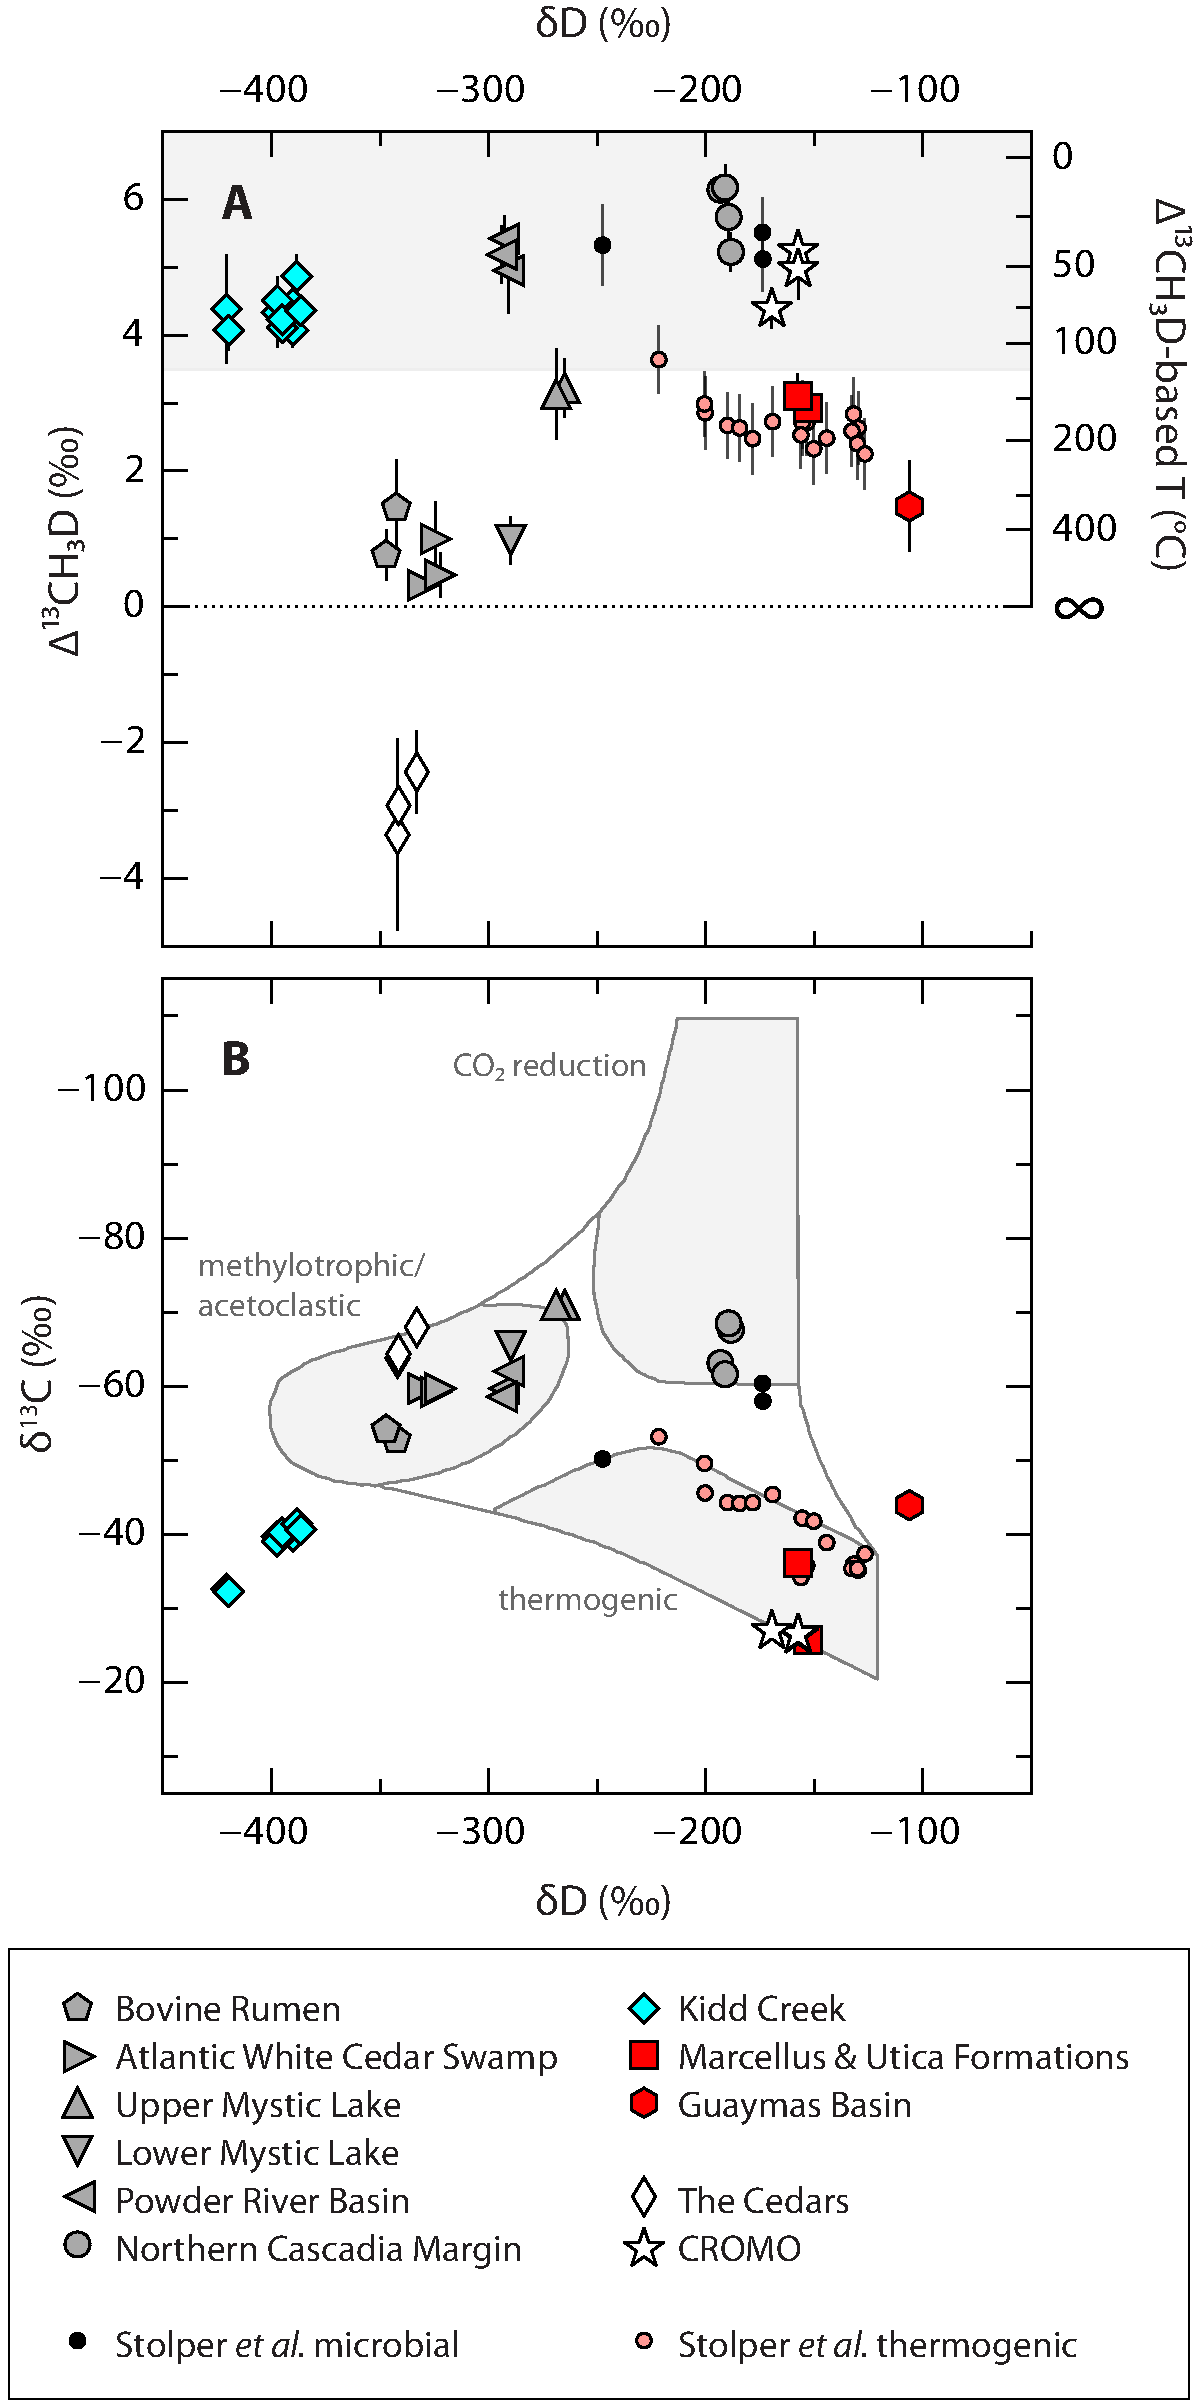
\includegraphics[width=0.5\linewidth]{figures/Fig2.1}
	\caption[Isotopologue compositions of methane samples from an environmental survey]{Isotopologue compositions of methane samples. \textbf{(A)}
	Δ\textsuperscript{13}CH\textsubscript{3}D plotted against δD. The
	Δ\textsuperscript{13}CH\textsubscript{3}D temperature scale corresponds
	to calibration in \autoref{fig:2:S1}. Error bars are 95\% confidence intervals
	(\autoref{tab:2:S1}). Data from \textcite{Stolper++_2014_S} were scaled to their
	corresponding Δ\textsuperscript{13}CH\textsubscript{3}D values
	\parencite{Stolper++_2014_GCA}. The shaded area represents the temperature range within
	which microbial life has been demonstrated to date \parencite{Takai++_2008_PNAS}. The
	hatched line represents Δ\textsuperscript{13}CH\textsubscript{3}D = 0‰ (\textit{T} → $\infty$); data plotting below this line cannot yield corresponding
	apparent temperatures. \textbf{(B)} δ\textsuperscript{13}C plotted
	against δD, showing characteristic fields for different methane sources
	from \textcite{Whiticar_1999_CG}.}
	\label{fig:2:1}
\end{SCfigure*}
